% Статья 1 (русская версия) — шаблон Springer Nature sn-article (стиль sn-mathphys-num).
% Целевой журнал: Minds and Machines (Springer).
\documentclass[sn-mathphys-num]{sn-jnl}

\usepackage{iftex}
\ifPDFTeX
\usepackage[T2A]{fontenc}
\usepackage[utf8]{inputenc}
\usepackage[russian,english]{babel}
\else
\usepackage{fontspec}
\defaultfontfeatures{Ligatures=TeX}
\setmainfont{DejaVu Serif}
\setsansfont{DejaVu Sans}
\setmonofont{DejaVu Sans Mono}
\usepackage[russian,english]{babel}
\fi
\usepackage{graphicx}
\usepackage{multirow}
\usepackage{amsmath,amssymb,amsfonts}
\usepackage{amsthm}
\usepackage{booktabs}
\usepackage{tabularx}
\usepackage{threeparttable}
\usepackage{xcolor}
\usepackage{url}

\graphicspath{{figures/}}

\raggedbottom

\newtheorem{theorem}{Теорема}
\newtheorem{corollary}[theorem]{Следствие}

\begin{document}

\selectlanguage{russian}

\title[Ограничения онтологической инновации в LLM]{Операциональные пределы онтологической инновации в больших языковых моделях: данные контролируемой генерации сенсорной модальности}

\author*[1]{\fnm{Jarno} \sur{Matarmaa}}\email{iarnoolavi.matarmaa@urfu.ru}
% \author[1]{\fnm{Second} \sur{Author}}\email{author2@urfu.ru}

\affil*[1]{\orgdiv{Институт радиоэлектроники и информационных технологий}, \orgname{Уральский федеральный университет}, \orgaddress{\city{Екатеринбург}, \country{Россия}}}

\abstract{%
Современные большие языковые модели порождают тексты, которые могут выглядеть концептуально новыми, что ставит вопрос о том, отражают ли такие ответы подлинную онтологическую инновацию --- введение концептов, невыразимых как рекомбинации или преобразования производных от обучающих данных примитивов, --- либо лишь сложную рекомбинацию внутри фиксированного репрезентационного многообразия. Мы рассматриваем этот вопрос в контролируемом эмпирическом исследовании, используя восьмимодальную мультимодальную сенсорную онтологию как экспериментальную вселенную. Семи моделям передового уровня (\textit{N}\,=\,168 предложений, по 24 прогона на модель) предлагалось предложить девятую сенсорную модальность, действительно выходящую за пределы заданных восьми. Ответы оценивались четырьмя конвергентными методами: трассируемостью в литературе с калиброванным порогом ($\tau = 0.40$), структурной декомпозицией, анализом выпуклой оболочки в пространстве эмбеддингов и непрерывной оценкой новизны. Результаты показывают нулевую строгую новизну $\hat{p}_{\mathrm{novel}}=0.000$ (95\% ДИ: [0.000, 0.000]), трассируемость $\hat{p}_{\mathrm{traceable}}=0.982$ и 100\% принадлежность выпуклой оболочке в эмбеддингах Sentence-BERT, редуцированных до трёх главных компонент. Структурная декомпозиция выявила три преобладающих режима неудачи: расширение диапазона (20.2\%), гибридная комбинация (44.6\%) и функциональная рекомбинация (17.9\%). Межмодельные эффекты умеренны ($\eta^{2}=0.305$), однако все модели остаются в одном низко-новизном режиме, что поддерживает объяснение через ограниченное многообразие, а не через дефицит конкретной модели. Мы интерпретируем результаты через \emph{теорему об отсутствии нового базиса} (No New Basis Theorem), устанавливающую, что обучение градиентным спуском при фиксированных словарях не может расширять репрезентационную размерность за пределы обучающих данных. Полученные данные систематически поддерживают позицию, согласно которой текущие нейросетевые архитектуры ограничены замыканием их обучающе-производных концептуальных пространств, с последствиями для операционализации и оценки онтологической креативности.
}

\keywords{онтологическая инновация, вычислительная креативность, большие языковые модели,
          концептуальные пространства, анализ трассируемости, репрезентационные ограничения}

\maketitle

% =========================================================================
\section{Введение}
\label{sec:intro}
% =========================================================================

Способность порождать принципиально новые концепты --- а не только рекомбинации уже имеющихся --- давно рассматривается как признак человеческого интеллекта и ключевой тест подлинной креативности. По мере того как большие языковые модели (LLM) демонстрируют впечатляющие результаты на всё более широком спектре генеративных задач, возникает важный вопрос: проявляют ли эти системы \emph{онтологическую инновацию}, то есть генерируют ли идеи за пределами концептуального замыкания их обучающей среды, или же они выступают исключительно мощными рекомбинаторами, ограниченными фиксированным репрезентационным многообразием?

Этот вопрос имеет и философскую, и практическую значимость. С философской точки зрения он связан с вычислительной теорией сознания, природой творчества и тем, могут ли алгоритмические системы в принципе выйти за пределы репрезентационных ресурсов, на которых они обучались. С практической точки зрения он определяет, какие роли большие языковые модели способны играть в научном открытии, проектировании и других областях, где требуются действительно новые концепты, а не просто новые компоновки уже известных элементов \cite{kuhn1962structure}.

Проблема в том, что ответы современных больших языковых моделей часто \emph{кажутся} новыми. Предложения, вводящие незнакомую терминологию, объединяющие концепты из разных дисциплин или описывающие механизмы, не представленные явно ни в одном отдельном обучающем документе, при поверхностной оценке могут выглядеть как подлинно креативные \cite{wiggins2006preliminary,colton2012computational}. Проверка того, являются ли такие ответы истинной концептуальной инновацией, требует контролируемого экспериментального дизайна и строгого многометодного анализа, а не оценки по внешнему впечатлению.

В этой статье мы представляем сфокусированное эмпирическое исследование, специально спроектированное для такой проверки. В качестве экспериментальной вселенной используется мультимодальная сенсорная онтология --- чётко определённое восьмимодальное концептуальное пространство, охватывающее биологическое и расширенное машинное восприятие. Такая постановка обеспечивает строгий контроль: мы точно знаем, какие концепты присутствуют в обучающем контексте, что позволяет систематически проверять, выходят ли сгенерированные ИИ предложения за пределы заданного пространства. Семи современным большим языковым моделям было предложено сформулировать \emph{девятую} сенсорную модальность, действительно выходящую за рамки исходных восьми. Оценка выполнялась четырьмя конвергентными методами, последовательно уточняющими диагностическую картину.

Наши основные вклады:

\begin{enumerate}
\item Контролируемая экспериментальная парадигма для операционализации онтологической инновации, основанная на чётко заданной мультимодальной сенсорной онтологии как явной обучающей вселенной.
\item Многометодная оценка, объединяющая трассируемость в литературе с калиброванными порогами, структурную декомпозицию, анализ выпуклой оболочки в пространстве эмбеддингов и непрерывный скоринг новизны, что даёт конвергентные данные без опоры на субъективное экспертное суждение.
\item Систематические эмпирические данные о том, что семь моделей передового уровня не производят строго новых предложений в 168 оценённых ответах при почти насыщенной трассируемости к известному концептуальному материалу.
\item Формальное обоснование через \emph{теорему об отсутствии нового базиса}, связывающее наблюдаемые эмпирические ограничения с архитектурными свойствами нейронных сетей, обученных градиентным спуском.
\end{enumerate}

Статья организована следующим образом. В разделе~\ref{sec:related} рассматриваются связанные работы по вычислительной креативности и репрезентационным ограничениям. Раздел~\ref{sec:methods} описывает датасет, задачу, модели и процедуры оценки. В разделе~\ref{sec:results} представлены результаты по всем методам. В разделе~\ref{sec:discussion} проводится интерпретация результатов, а в разделе~\ref{sec:limits} обсуждаются ограничения исследования.

% =========================================================================
\section{Теоретический контекст и связанные работы}
\label{sec:related}
% =========================================================================

\subsection{Таксономия креативности Боден}

Доминирующей рамкой анализа машинной креативности остаётся трипартидная таксономия Маргарет Боден \cite{boden2004creative}, различающая типы результатов по их отношению к концептуальному пространству, из которого они возникают. \emph{Комбинаторная креативность} порождает новые сочетания знакомых идей --- поэтические метафоры, аналогии, концептуальные бленды. \emph{Исследовательская креативность} систематически обходит хорошо определённые концептуальные пространства, находя ранее не посещённые области. \emph{Трансформационная креативность}, наиболее радикальная категория, модифицирует само концептуальное пространство, ослабляя или изменяя его определяющие ограничения.

Исследования систем искусственного интеллекта демонстрируют существенную компетентность в комбинаторной и исследовательской креативности \cite{hofstadter1995fluid,cope1996experiments}. Системы вроде Copycat, JAPE и AARON способны порождать результаты, которые люди-оценщики считают действительно неожиданными и уместными в соответствующих доменах. Устойчивая трансформационная креативность при этом остаётся редкой: большинство задокументированных примеров касается поверхностных модификаций параметров, а не фундаментальной реконцептуализации \cite{boden2004creative}.

Wiggins \cite{wiggins2006preliminary} предложил формальную схему оценки заявлений о креативности и выделил проблему «рамки» (framing): системы могут казаться трансформирующими своё концептуальное пространство, фактически действуя внутри неявно более широкого пространства, заданного людьми-разработчиками. Эта критика особенно актуальна для современных больших языковых моделей, чьи обучающие корпуса неявно задают огромную, но всё же конечную концептуальную вселенную.

\subsection{Наше расширение: онтологическая креативность}

Мы утверждаем, что для описания наиболее радикальной формы концептуальной инновации необходима четвёртая категория, которую мы называем \emph{онтологической креативностью}. Трансформационная креативность изменяет операторы $\Omega$ или отношения $\mathcal{E}$ в концептуальном пространстве $\mathcal{C} = (V, \mathcal{E}, \Phi, \Omega)$; онтологическая креативность вводит новые \emph{примитивные} концепты $v' \in V'$ при условии $V' \not\subset V$, и критически важно, что $V'$ не может быть выражено как $\Omega(V)$ для любых существующих операторов.

Это различие согласуется с философским понятием категориальной ошибки у Райла \cite{ryle1949concept}: онтологическая креативность предполагает распознавание недостаточности существующих категорий и выдвижение новых, не сводимых к рекомбинации или трансформации текущих примитивов. Реконцептуализация абсолютной одновременности у Эйнштейна как категориальной ошибки, приведшая к новой онтологии релятивистского пространства-времени, является примером именно такого типа креативности. Аналогично, предложение действительно новой сенсорной модальности должно быть не расширением и не гибридом известных, а типом восприятия с физическим основанием и информационным содержанием, невыразимым как композиция текущих восьми.

\subsection{Формальные репрезентационные ограничения}

Вычислительная теория сознания \cite{turing1936computable,godel1931formal} и её критики \cite{searle1980minds,penrose1990emperors,dreyfus1972computers} давно обсуждают, существуют ли принципиальные пределы того, что алгоритмические системы могут представлять и понимать. Недавние работы по механистической интерпретируемости дают эмпирическую опору этой дискуссии, показывая, что генерация в трансформерных больших языковых моделях реализуется как извлечение и интерполяция между примерами из обучения, а не как механизм вывода, способный вводить принципиально новые примитивы \cite{brown2020language,elhage2021mathematical}. Архитектура трансформера \cite{vaswani2017attention} кодирует знание неявно в весах, выученных на статистике совместной встречаемости, что привязывает пространство выходов к обучающему словарю концептов. Формализм концептуальных пространств Гэрденфорса \cite{gardenfors2000conceptual} даёт комплементарную геометрическую интуицию: выученный концепт представлен как область в пространстве качеств, и генерация нового концепта вне всех существующих областей требует внешнего базисного вектора, отсутствующего в обучающих данных.

Мы формализуем это ограничение как \emph{теорему об отсутствии нового базиса}: для любой нейроархитектуры $\mathcal{A}$, работающей в репрезентационном пространстве $\mathbb{R}^{d}$, с генеративным процессом $G\colon \mathbb{R}^{d} \to \mathbb{R}^{d}$, обученным на данных $\mathcal{D} = \{x_1,\ldots,x_N\}$, все сгенерированные ответы $x' = G(z)$ лежат в $\mathcal{M}'$, непрерывной деформации $\mathcal{M} = \mathrm{span}(\{x_1,\ldots,x_N\})$, удовлетворяющей $\dim(\mathcal{M}') \leq \dim(\mathcal{M})$. Онтологическая новизна требовала бы расширения базиса $\mathcal{M}$, чего никакой внутренний генеративный механизм не может достичь без архитектурного или датасетного расширения.

Эта теорема объясняет, почему даже очень сильные модели, способные к неожиданным комбинациям, формально остаются ограничены концептуальной вселенной, определяемой их обучающими данными. Наше эмпирическое исследование даёт контролируемую проверку того, проявляется ли это теоретическое ограничение в поведении моделей.

\subsection{Проблемы оценки в вычислительной креативности}

Устойчивая методологическая проблема исследований вычислительной креативности --- это оценка \cite{wiggins2006preliminary,colton2012computational}. Экспертные человеческие суждения субъективны, плохо воспроизводимы и чувствительны к эффектам рамки. Недавние исследования показывают, что большие языковые модели могут достигать уровня человека в задачах дивергентного мышления, например в Alternative Uses Test \cite{stevenson2022gpt}, однако качество оценок сильно зависит от выбранной метрики \cite{organisciak2023beyond}. Работы 2024--2026 гг. дополнительно подтверждают чувствительность результатов к выбранному протоколу и предлагают новые схемы оценки креативности LLM, включая human-comparative, temperature-sensitivity и model-guided judging подходы \cite{zhao2024assessing,wang2024canai,peeperkorn2024temperature,bellemare2024divergent,ismayilzada2024shortstory,nakajima2026beyonddivergent,olson2024steering}. Наш многометодный подход --- поиск трассируемости, структурная декомпозиция, геометрия пространства эмбеддингов и непрерывная оценка --- даёт конвергентные автоматизированные данные, которые можно воспроизводить и расширять. Калиброванные пороги трассируемости заменяют произвольные отсечки эмпирически обоснованными рабочими точками.

% =========================================================================
\section{Материалы и методы}
\label{sec:methods}
% =========================================================================

\subsection{Мультимодальная сенсорная онтология}

Экспериментальная вселенная состоит из восьми сенсорных модальностей, каждая из которых определена физическим основанием, информационным каналом и функциональной ролью во взаимодействии агента с окружающей средой (таблица~\ref{tab:modalities}). Модальности охватывают как биологические человеческие чувства, так и расширенные возможности машинного восприятия:

\begin{table}[tp]
\caption{Восьмимодальная сенсорная онтология, использованная как экспериментальная вселенная исследования. Каждая модальность определена физическим основанием, репрезентационной размерностью и функциональной ролью.}
\label{tab:modalities}
\begin{tabularx}{\textwidth}{lXXr}
\toprule
\textbf{Модальность} & \textbf{Физическое основание} & \textbf{Функциональная роль} & \textbf{Размерн.} \\
\midrule
Визуальная       & ЭМ-спектр 300--1000\,нм (шаг 5\,нм) & Распознавание сцены и объектов & 140 \\
Аудиторная       & Волны давления 1\,Гц--100\,кГц (128-бинное БПФ) & Локализация источников звука & 128 \\
Тактильная       & Механические вибрации 5--800\,Гц & Текстура поверхности и давление & 32 \\
Обонятельная     & Химические категории (10 классов) & Идентификация веществ & 10 \\
Вкусовая         & Вкусовые измерения (сладкий/кислый/солёный/горький/умами) & Навигация потребления & 5 \\
Проприоцептивная & 20 углов суставов + 10 мышечных напряжений & Оценка состояния тела & 30 \\
Вестибулярная    & 3-осевое ускорение + 3-осевая угловая скорость & Баланс и движение & 6 \\
Интероцептивная  & ЧСС, дыхание, кожная проводимость, температура, голод, жажда, усталость, боль & Гомеостатическая регуляция & 8 \\
\midrule
\multicolumn{3}{l}{\textit{Суммарная размерность признаков на временной шаг}} & 359 \\
\bottomrule
\end{tabularx}
\end{table}

Полный датасет содержит 5000 обучающих, 1000 валидационных и 1000 тестовых примеров; каждый пример представляет 60-секундный эпизод с дискретизацией 1\,Гц (21\,540 точек данных на пример), сформированный в семи повседневных сценариях (ходьба, бег, сидение, еда, питьё, прослушивание, визуальное наблюдение). Явный машиночитаемый слой онтологии документирует физическое основание, информационное содержание и функциональную роль каждой модальности, что делает возможной автоматизированную оценку.

\subsection{Определение задачи и контракт промпта}

Каждой модели предлагалось \emph{предложить девятую сенсорную модальность, действительно новую и не сводимую к комбинациям, расширениям или трансформациям существующих восьми}. Предложения должны были указывать: (1) физический феномен, который следует воспринимать, (2) информационный канал и кодирование, (3) функциональное отличие от существующих модальностей. Полная таблица онтологии (таблица~\ref{tab:modalities}) предоставлялась в структурированном табличном формате вместе с естественно-языковым описанием каждой модальности.

Промпты проектировались как нейтральные к задаче: они не подсказывали, какие ответы считаются новыми или неновыми, чтобы избежать якорения моделей на определённые типы ответов. Для каждой из семи моделей было собрано по 24 независимых прогона, всего $N = 7 \times 24 = 168$ предложений.

\subsection{Модели и реализация}

Оценивались семь моделей передового уровня: GPT-5.2 \cite{openai2023gpt4}, Claude-3.7-Sonnet, Gemini-3.1-Pro-Preview \cite{gemini15_2024}, LLaMA-3.3-70B-Instruct \cite{llama3herd_2024}, DeepSeek-v3.2 \cite{deepseekv3_2024,deepseekr1_2025}, Mistral-Large \cite{mixtral2024} и Perplexity Sonar Pro; доступ осуществлялся через API OpenRouter, Perplexity и Mistral. Во всех запусках использовалась температура $T=0.7$; API Perplexity не поддерживает настройку температуры и работал с параметрами по умолчанию провайдера. Системные запросы были сформулированы нейтрально, чтобы представить задачу без смещения в сторону конкретных типов ответов.

\subsection{Протокол оценки}

\paragraph{Трассируемость в литературе.}
Каждое предложение сопоставлялось с курируемым научным корпусом из 125 документов по сенсорной биологии, робототехническому сенсингу и вычислительной нейронауке с использованием косинусного сходства эмбеддингов Sentence-BERT \cite{reimers2019sentencebert}. Предложение классифицировалось как \emph{трассируемое}, если его максимальное сходство с документом превышало порог $\tau$.

Выбор порога выполнялся в явном калибровочном шаге. Три кандидатные рабочие точки ($\tau \in \{0.30, 0.40, 0.50\}$) сравнивались на полном распределении сходства «ответ--корпус». При $\tau=0.30$ все предложения оказывались трассируемыми (в среднем 23.7 совпадающих документов на предложение), что не даёт дискриминации. При $\tau=0.50$ трассируемыми оставались лишь 64.9\% предложений (в среднем 1.24 совпадения), что указывает на чрезмерное отсечение. Промежуточное значение $\tau=0.40$ выбрано как наиболее обоснованная рабочая точка: 98.2\% трассируемости при среднем 7.36 совпадения выше порога на предложение, то есть с сохранением дискриминации и без вырождения к крайним режимам.

\paragraph{Структурная декомпозиция.}
Каждое предложение анализировалось на предмет того, можно ли его ключевые утверждения выразить через восемь обучающих примитивов с помощью: (i) расширения диапазона (сохранение типа восприятия при сдвиге физического параметрического диапазона), (ii) гибридной комбинации (объединение признаков двух и более существующих модальностей), (iii) функциональной рекомбинации (переназначение существующего сенсорного механизма на другую функциональную роль). Предложения, не попадающие ни в одну категорию, маркировались как \emph{структурно новые}.

\paragraph{Анализ выпуклой оболочки в пространстве эмбеддингов.}
Для каждого предложения и для описаний восьми обучающих модальностей вычислялись эмбеддинги Sentence-BERT. Метод главных компонент редуцировал оба набора до трёх компонент; принадлежность выпуклой оболочке в 3D определялась через уравнения полупространств с численной толерантностью. Классификация предложения как \emph{вне} оболочки означала бы размещение в семантически изолированной области, что могло бы указывать на расширение базиса за пределы обучающей онтологии.

\paragraph{Непрерывная оценка новизны.}
Для каждого предложения вычислялся непрерывный балл новизны $s \in [0,1]$, комбинирующий структурные подоценки: (i) отсутствие попадания в категории структурной декомпозиции, (ii) обратную величину максимального косинусного сходства с обучающими модальностями, (iii) геометрическую дистанцию до границы выпуклой оболочки. Предложения с $s \geq 0.5$ классифицировались как строго новые по выбранному операциональному порогу.

% =========================================================================
\section{Результаты}
\label{sec:results}
% =========================================================================

\subsection{Основные результаты}

Итоговая доля строгой новизны составила $\hat{p}_{\mathrm{novel}} = 0.000$ (95\% ДИ: [0.000, 0.000]; $N=168$). Ни одно предложение не удовлетворило критерию строгой новизны $s \geq 0.5$. Средний непрерывный балл новизны равен $\hat{\mu}_{\mathrm{continuous}} = 0.059$ (SD $= 0.031$), что указывает на слабый сигнал новизны без пороговых событий во всех моделях и прогонах.

При калиброванном пороге трассируемости $\tau = 0.40$ доля трассируемых предложений составила $\hat{p}_{\mathrm{traceable}} = 0.982$ (95\% ДИ: [0.962, 1.000]); 165 из 168 предложений имели максимальное косинусное сходство выше порога, средний лучший матч по всем предложениям равен 0.528. Из 165 трассируемых предложений все 165 сопоставлены с источниками из сильного уровня доказательности корпуса.

На рисунке~\ref{fig:classification} показано доминирующее распределение классов: трассируемые и неновые ответы подавляюще преобладают во всех моделях.

\begin{figure}[tp]
\centering
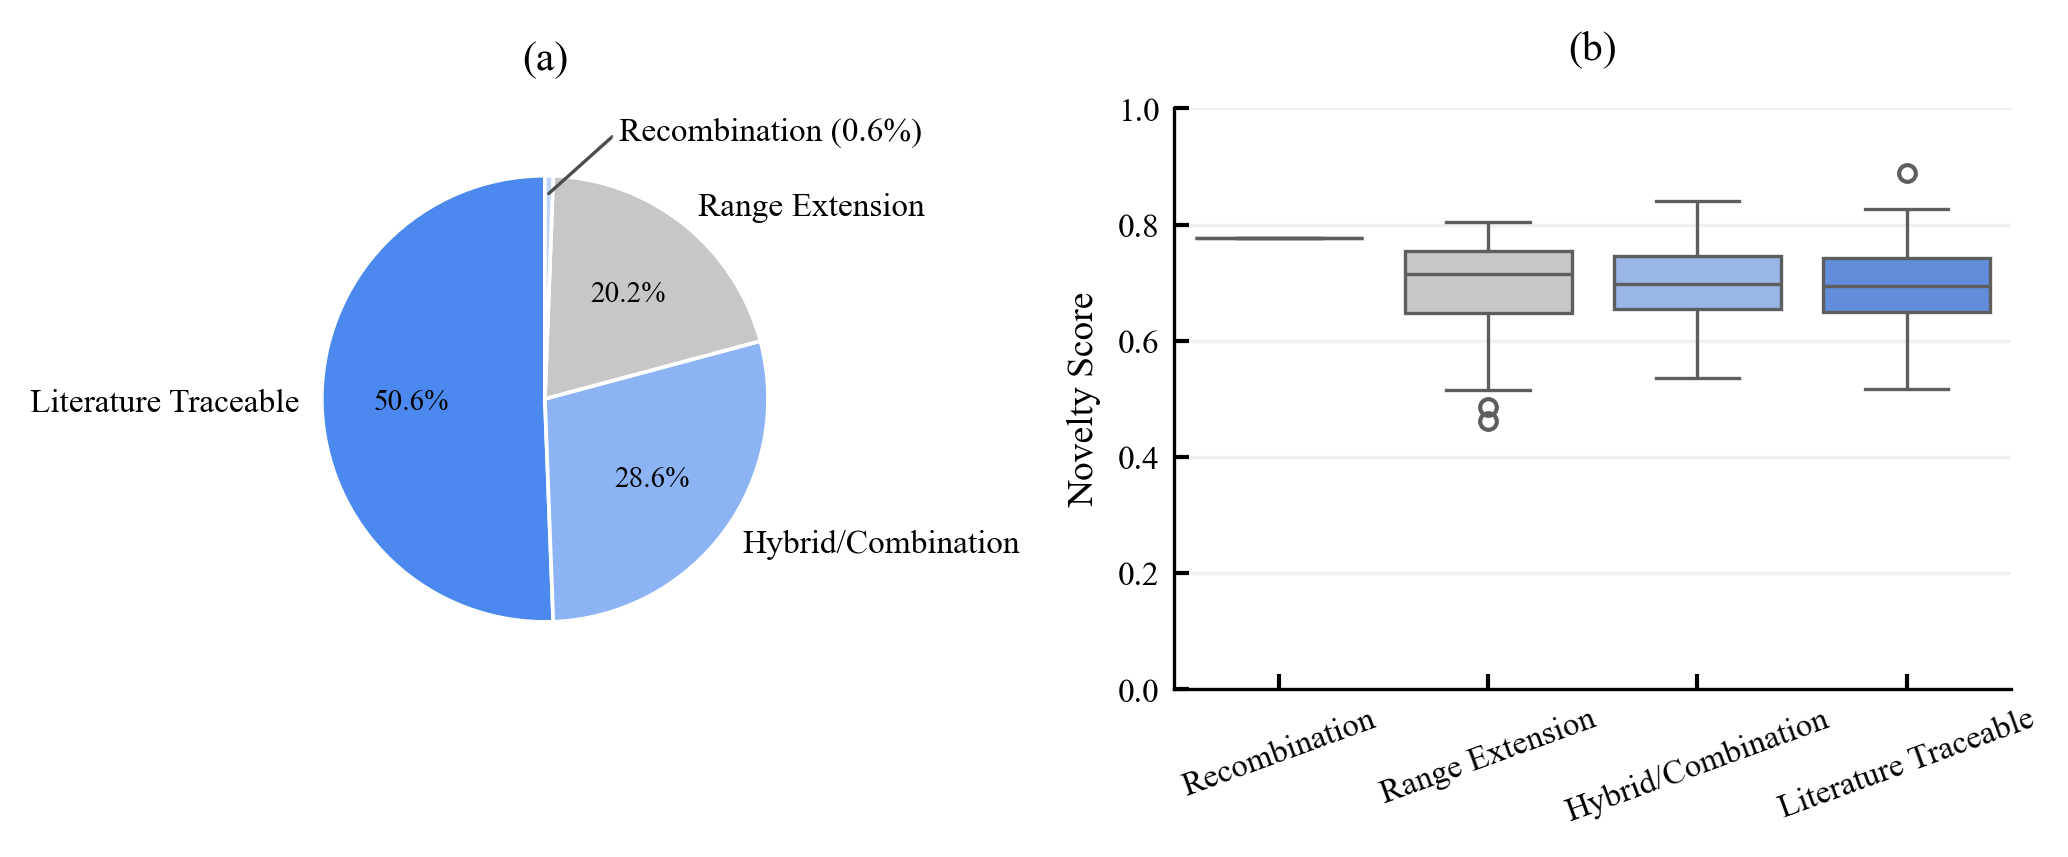
\includegraphics[width=\textwidth]{t1_classification_summary.png}
\caption{Сводка классификации предложений ($N=168$ предложений, семь моделей).
(a)~Распределение исходов классификации; распределение доминируется трассируемыми категориями, согласующимися с низкой операциональной онтологической новизной при калиброванных порогах.
(b)~Распределения баллов новизны по категориям классификации (box plot).}
\label{fig:classification}
\end{figure}

\subsection{Структурная декомпозиция}

Из 168 предложений 88 (52.4\%) оказались структурно декомпозируемыми в примитивы обучающей онтологии. Эти предложения объясняются тремя типами неудачи:

\begin{itemize}
\item \textbf{Расширение диапазона} (34 случая, 20.2\%): предложения, расширяющие физический параметрический диапазон существующей модальности (например, дальний инфракрасный термальный сенсинг как расширение визуального ЭМ-диапазона или расширенное в инфразвук аудиторное обнаружение).
\item \textbf{Гибридная комбинация} (75 случаев, 44.6\%): предложения, объединяющие признаки двух и более существующих модальностей (например, комбинированное тактильно-проприоцептивное «haptic flow»-восприятие или обонятельно-вкусовая интеграция).
\item \textbf{Функциональная рекомбинация} (30 случаев, 17.9\%): предложения, переиспользующие существующий сенсорный механизм для иной функциональной роли (например, применение интероцептивных сигналов для мониторинга внешней среды, а не гомеостатической регуляции).
\end{itemize}

Оставшиеся 80 предложений (47.6\%) не декомпозировались полностью через три именованные категории, но всё равно попадали в порог трассируемости, что указывает на семантическую близость к известным концептам даже без простого пути структурной декомпозиции.

На рисунке~\ref{fig:frontier_bands} показаны распределения по полосам границы новизны для каждой модели: паттерн низкой новизны и высокой трассируемости воспроизводится на уровне всех архитектур и не сводится к одной слабой модели. Рисунок~\ref{fig:frontier_decomp} дополнительно демонстрирует, что большинство предложений одновременно нарушают несколько критериев границы новизны, поддерживая интерпретацию сопряжённых ограничений.

\begin{figure}[tp]
\centering
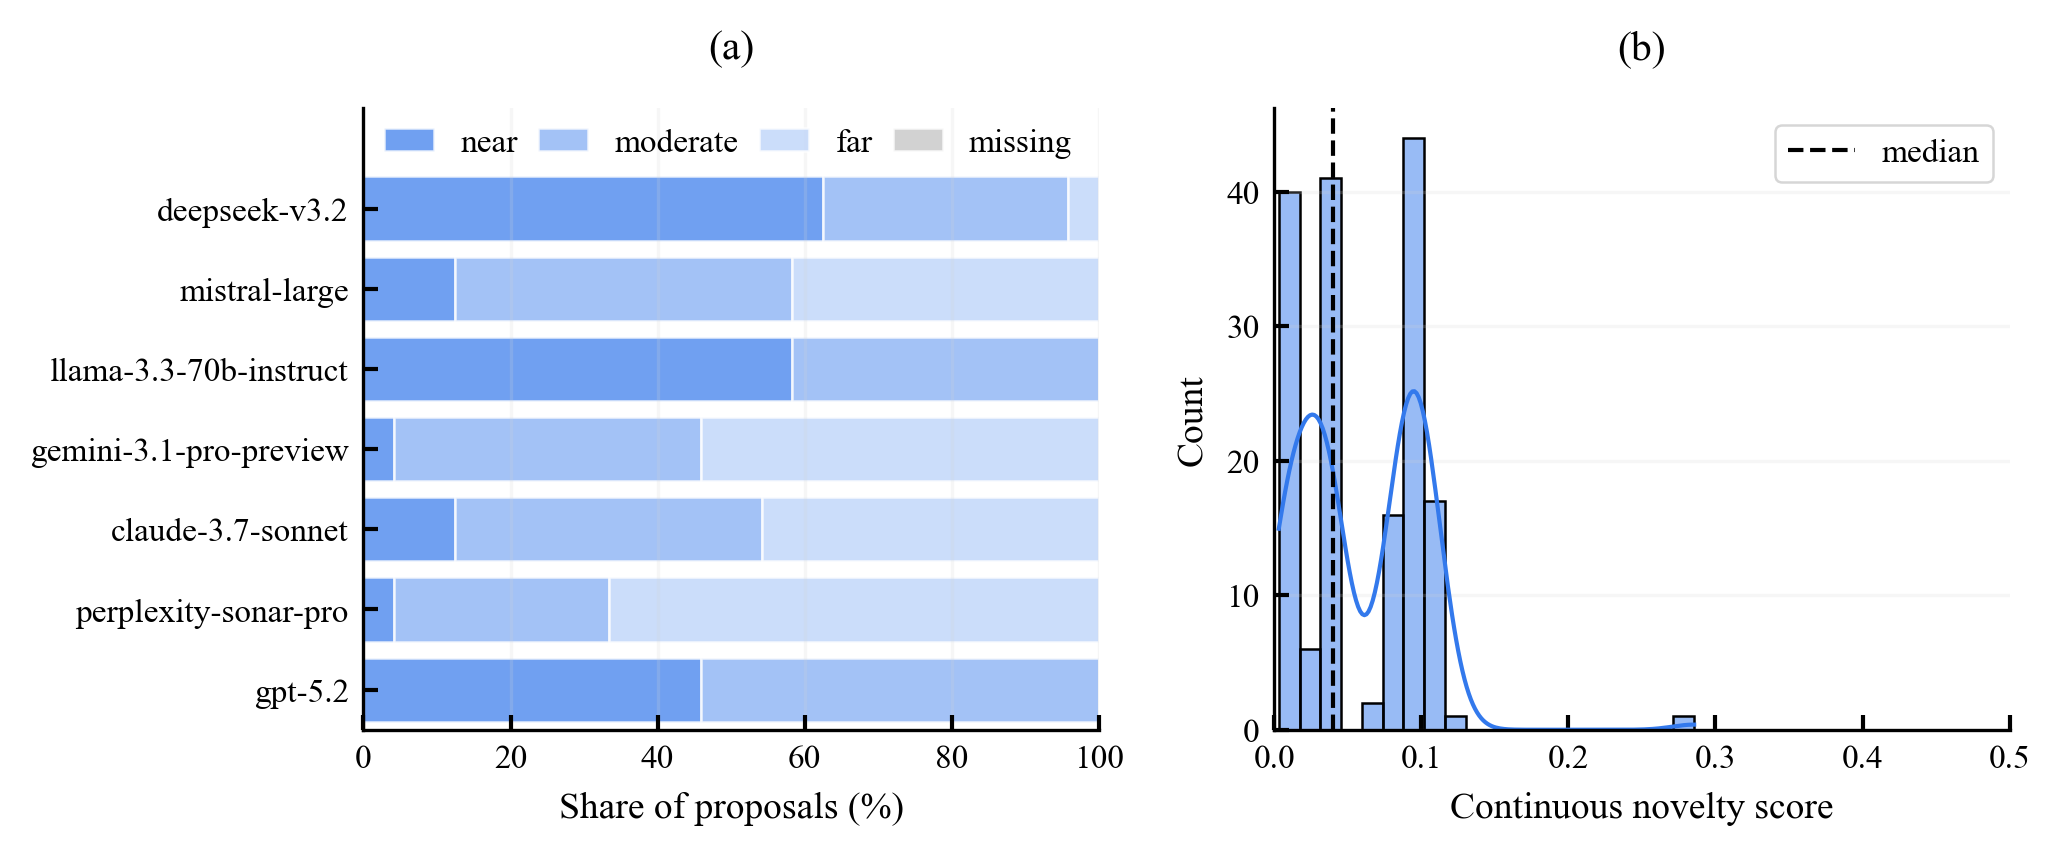
\includegraphics[width=\textwidth]{t1_novelty_frontier_bands_by_model.png}
\caption{Распределения по полосам границы новизны и распределение баллов.
(a)~Распределения полос по моделям: ответы концентрируются в зонах низкой новизны и близости к границе новизны во всех семи архитектурах, что указывает на архитектурно-независимые паттерны ограничений, а не на изолированные провалы конкретных моделей.
(b)~Общее распределение непрерывного балла новизны с наложением оценки плотности; пунктирная линия показывает медиану.}
\label{fig:frontier_bands}
\end{figure}

\begin{figure}[tp]
\centering
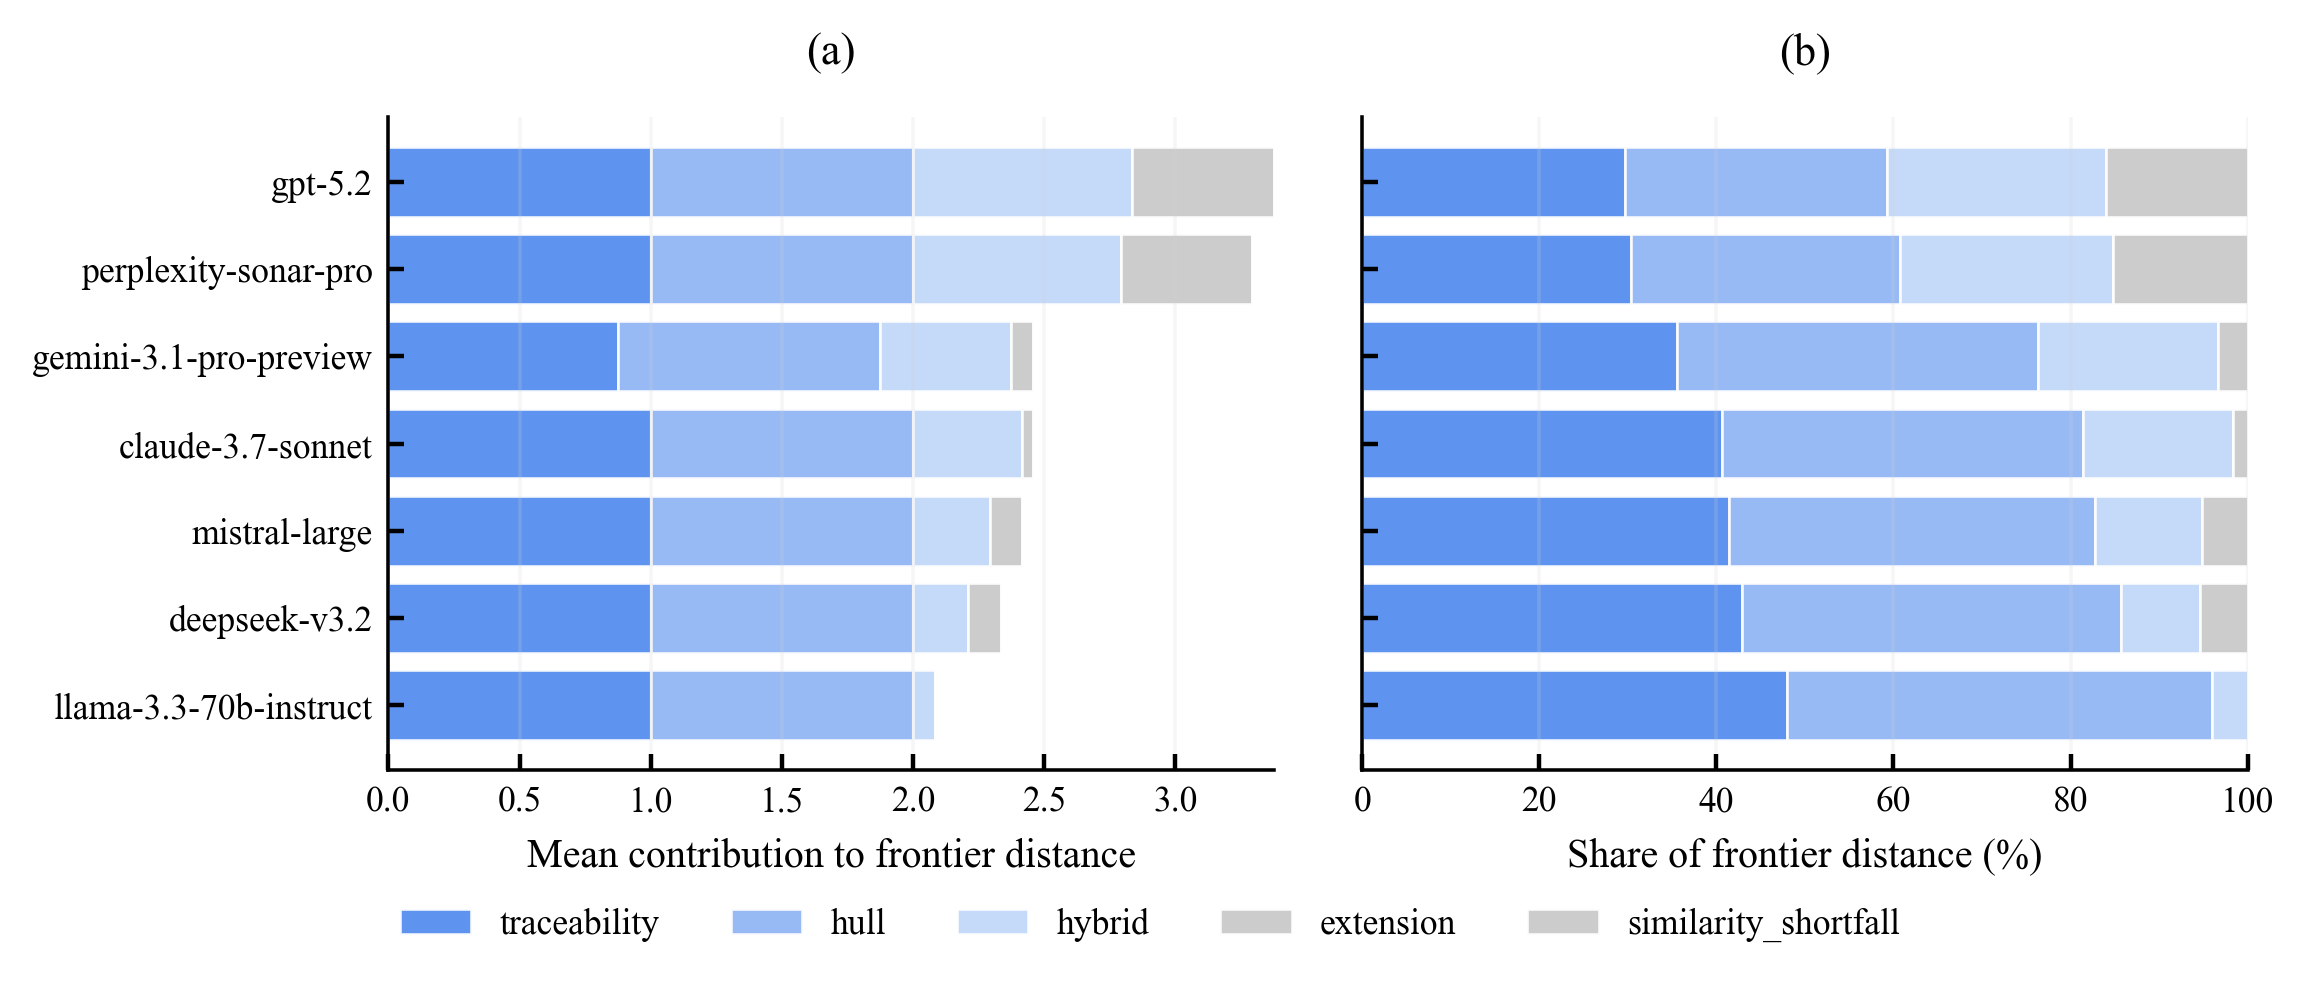
\includegraphics[width=\textwidth]{t1_novelty_frontier_decomposition_by_model_combined.png}
\caption{Декомпозиция критериев границы новизны по моделям.
(a)~Абсолютный средний вклад каждого критерия в общую дистанцию до границы новизны.
(b)~Относительная доля (\%) дистанции до границы новизны по критериям.
Обе панели подтверждают, что большинство ответов нарушают несколько критериев одновременно, что поддерживает интерпретацию сопряжённых ограничений низкой онтологической новизны.}
\label{fig:frontier_decomp}
\end{figure}

\subsection{Геометрия пространства эмбеддингов}

Все 168 предложений (100\%) классифицированы как находящиеся внутри 3D выпуклой оболочки эмбеддингов обучающих модальностей. Точки предложений кластеризуются во внутренней области обучающего многообразия; ни одно предложение не занимает семантически изолированную область, которая указывала бы на расширение базиса за пределы обучающей онтологии.

Среднее косинусное сходство между каждым предложением и ближайшей обучающей модальностью составило $\bar{d} = 0.305$ (SD $= 0.078$), что указывает на существенное семантическое перекрытие с обучающими концептами. На рисунке~\ref{fig:embedding} представлена визуализация анализа пространства эмбеддингов: предложения показаны в первых двух главных компонентах, а граница 3D оболочки дана как визуальный ориентир.

\begin{figure}[tp]
\centering
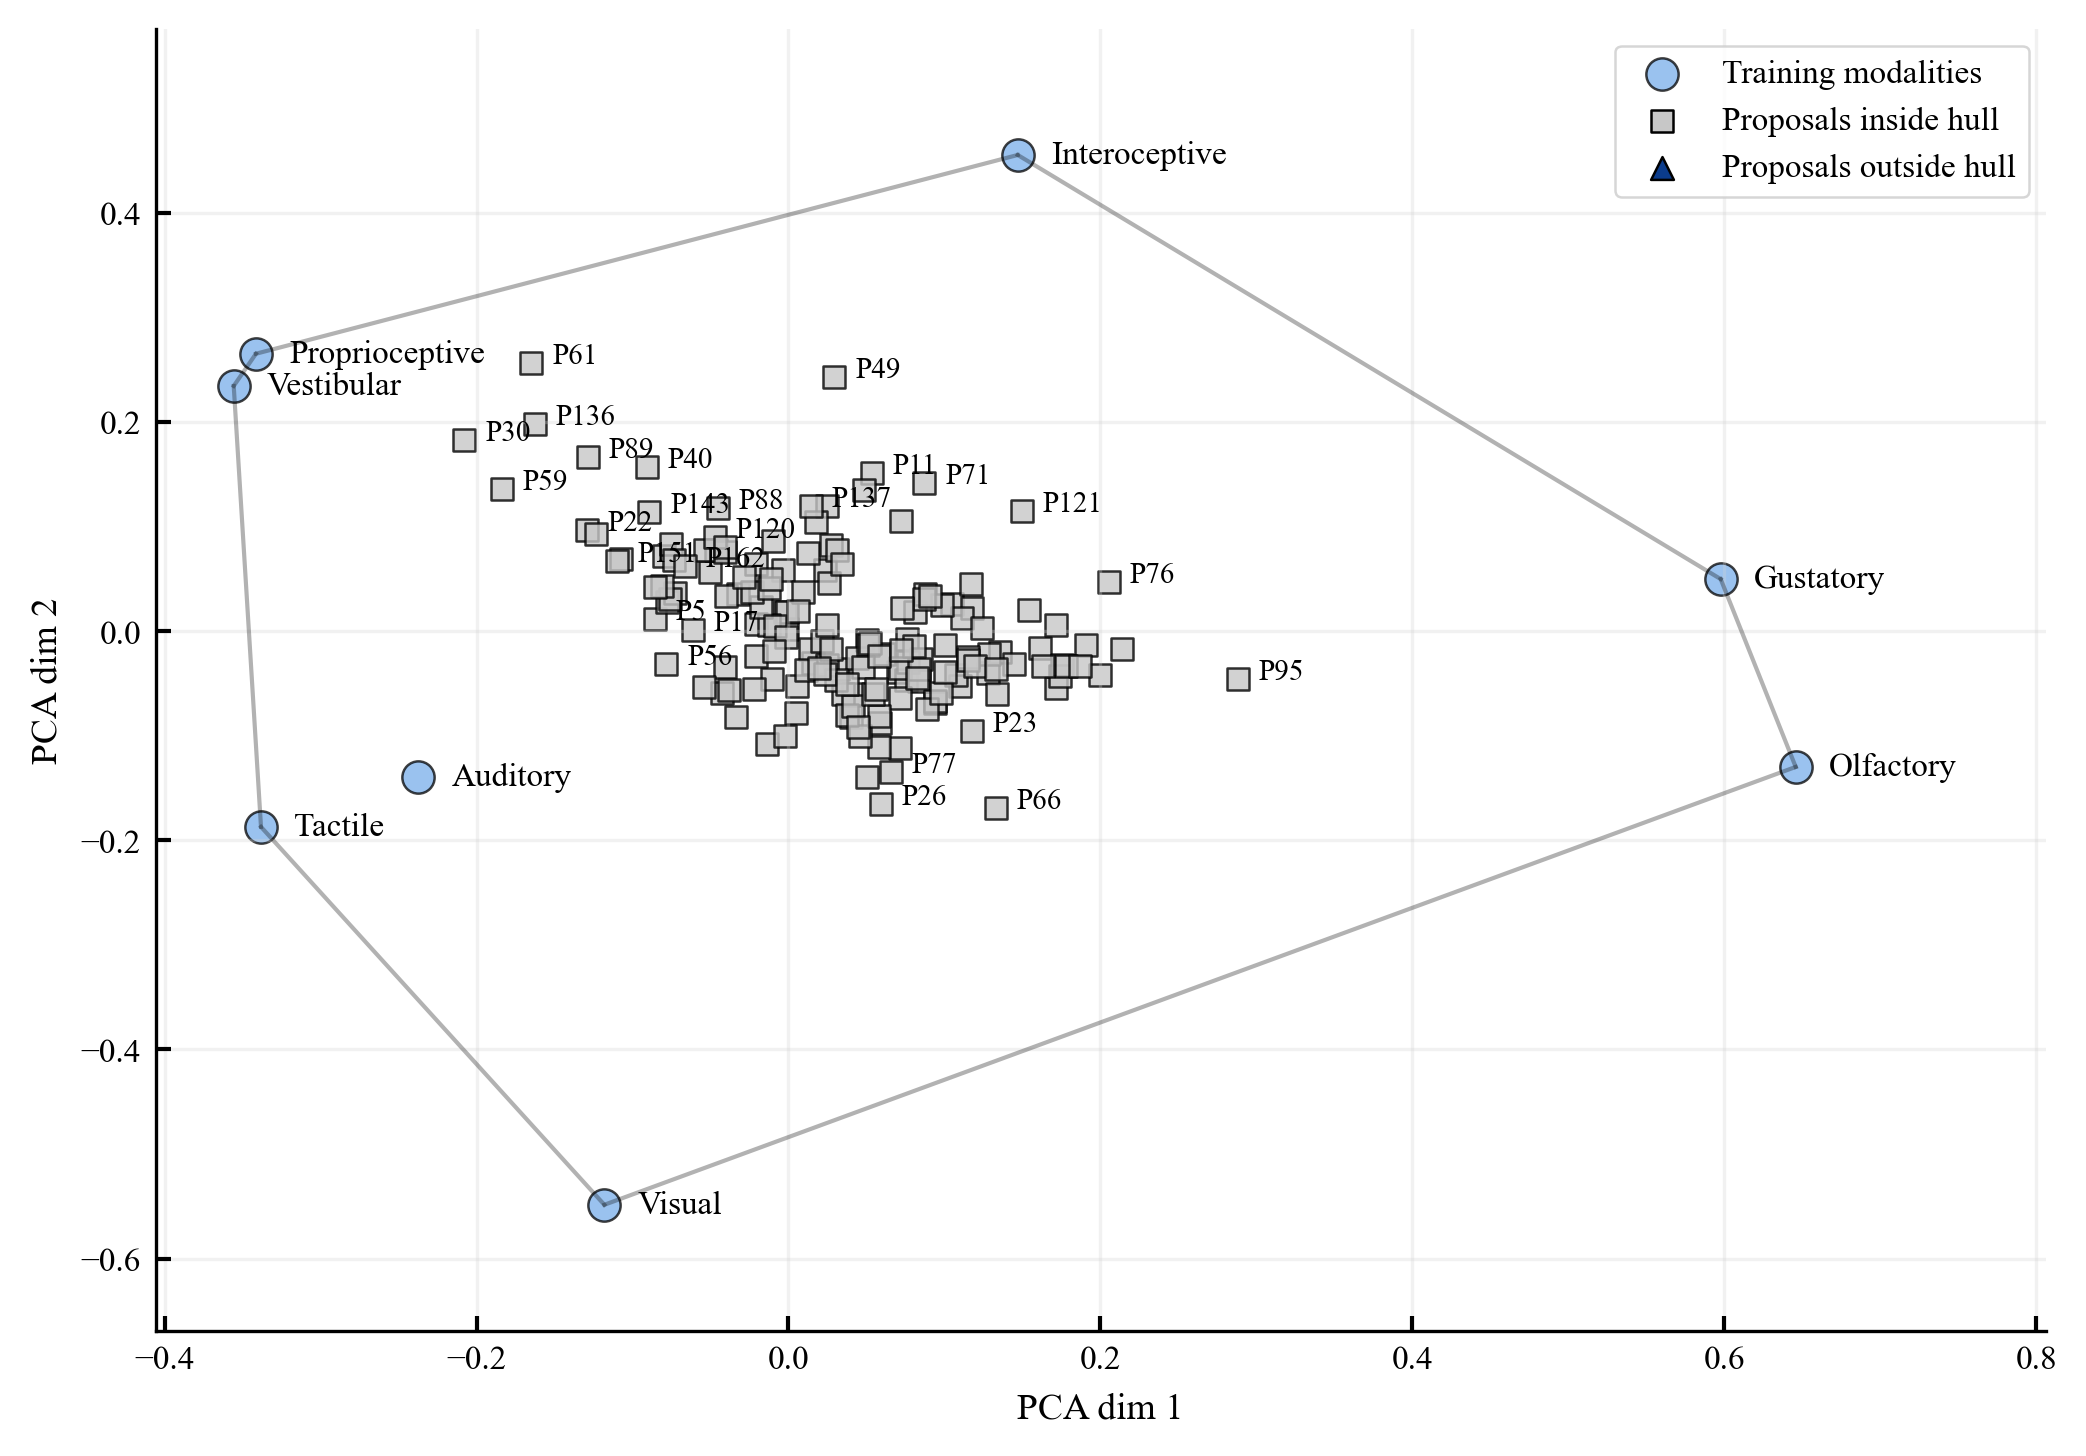
\includegraphics[width=\textwidth]{t1_embedding_space_analysis.png}
\caption{Анализ пространства эмбеддингов для предложений эксперимента и обучающих модальностей. Принадлежность выпуклой оболочке вычисляется в PCA-редуцированном 3D пространстве; показанная 2D граница носит иллюстративный характер. Все 168 точек предложений кластеризуются рядом с внутренней частью обучающего многообразия --- ни одна не выходит в семантически изолированную область.}
\label{fig:embedding}
\end{figure}

Рисунок~\ref{fig:similarity_heatmap} показывает агрегированную тепловую карту косинусного сходства между предложенными и восемью обучающими модальностями и приводит к тому же выводу по комплементарной метрике: каждое предложение демонстрирует повышенное сходство хотя бы с одной обучающей модальностью; нет предложений с равномерно низким сходством со всеми восемью.

\begin{figure}[tp]
\centering
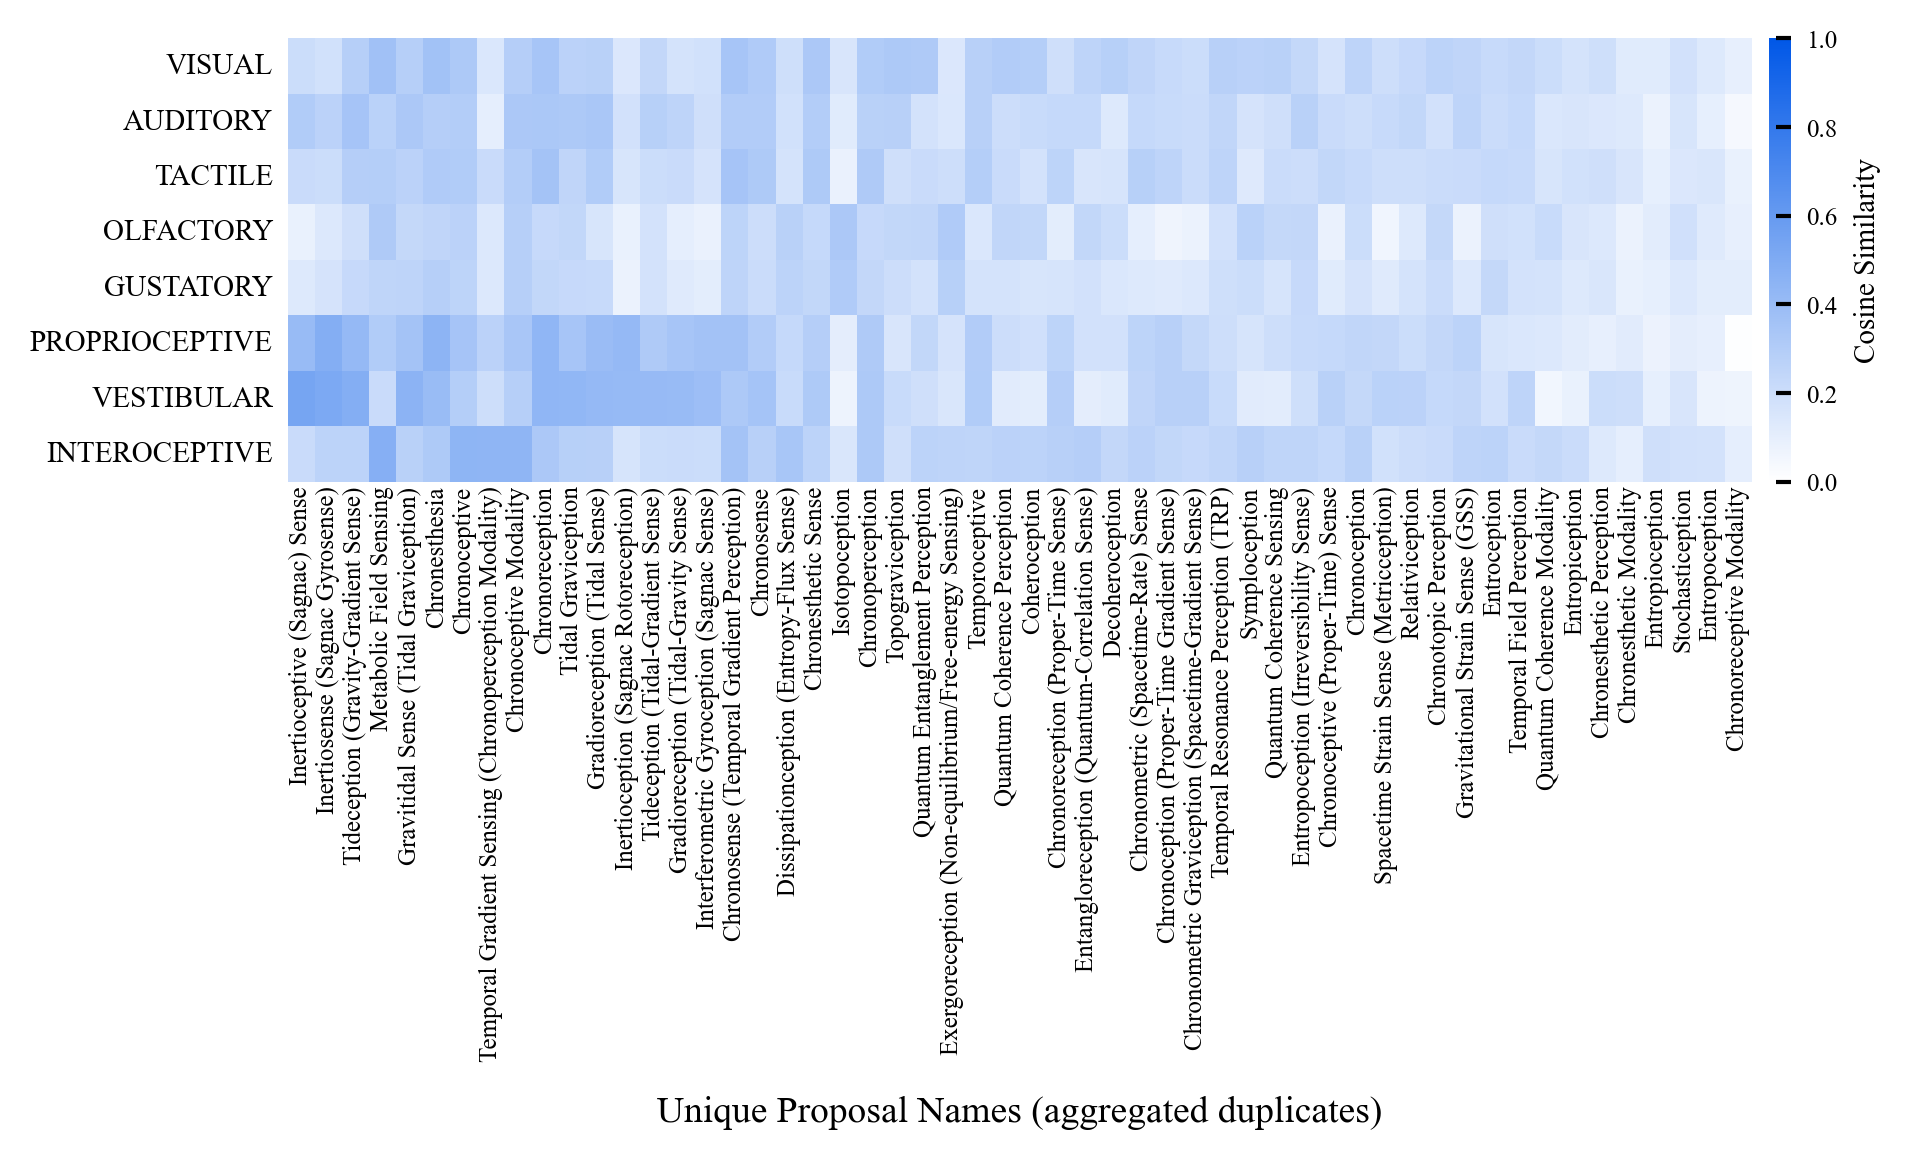
\includegraphics[width=\textwidth]{t1_similarity_heatmap_v1_optionA_aggregated.png}
\caption{Агрегированное косинусное сходство предложенных модальностей с восьмью обучающими модальностями. Концентрация значений сходства подтверждает вывод о трассируемости: нет ни одного предложения, одновременно несходного со всеми восемью обучающими типами.}
\label{fig:similarity_heatmap}
\end{figure}

\subsection{Сравнение моделей}

Модельный эффект по основной метрике новизны оказался умеренным: однофакторный дисперсионный анализ (ANOVA) дал $\eta^{2} = 0.305$, что указывает на нетривиальную межмодельную вариативность «сырых» баллов. Тем не менее все семь моделей остаются в одном режиме низкой новизны и высокой трассируемости: ни одна модель не породила предложений, классифицированных как строго новые, и ни одна не достигла среднего непрерывного балла новизны выше $\mu = 0.12$.

На рисунке~\ref{fig:canonical_heatmap} показано, что межмодельная вариативность проявляется как различия в \emph{предпочтениях среди известных канонических семейств}, а не как возникновение структурно новых семейств: одни модели чаще генерируют расширения диапазона, другие --- гибридные комбинации, но ни один паттерн не означает выхода за пределы обучающе-производного многообразия.

\begin{figure*}[tp]
\centering
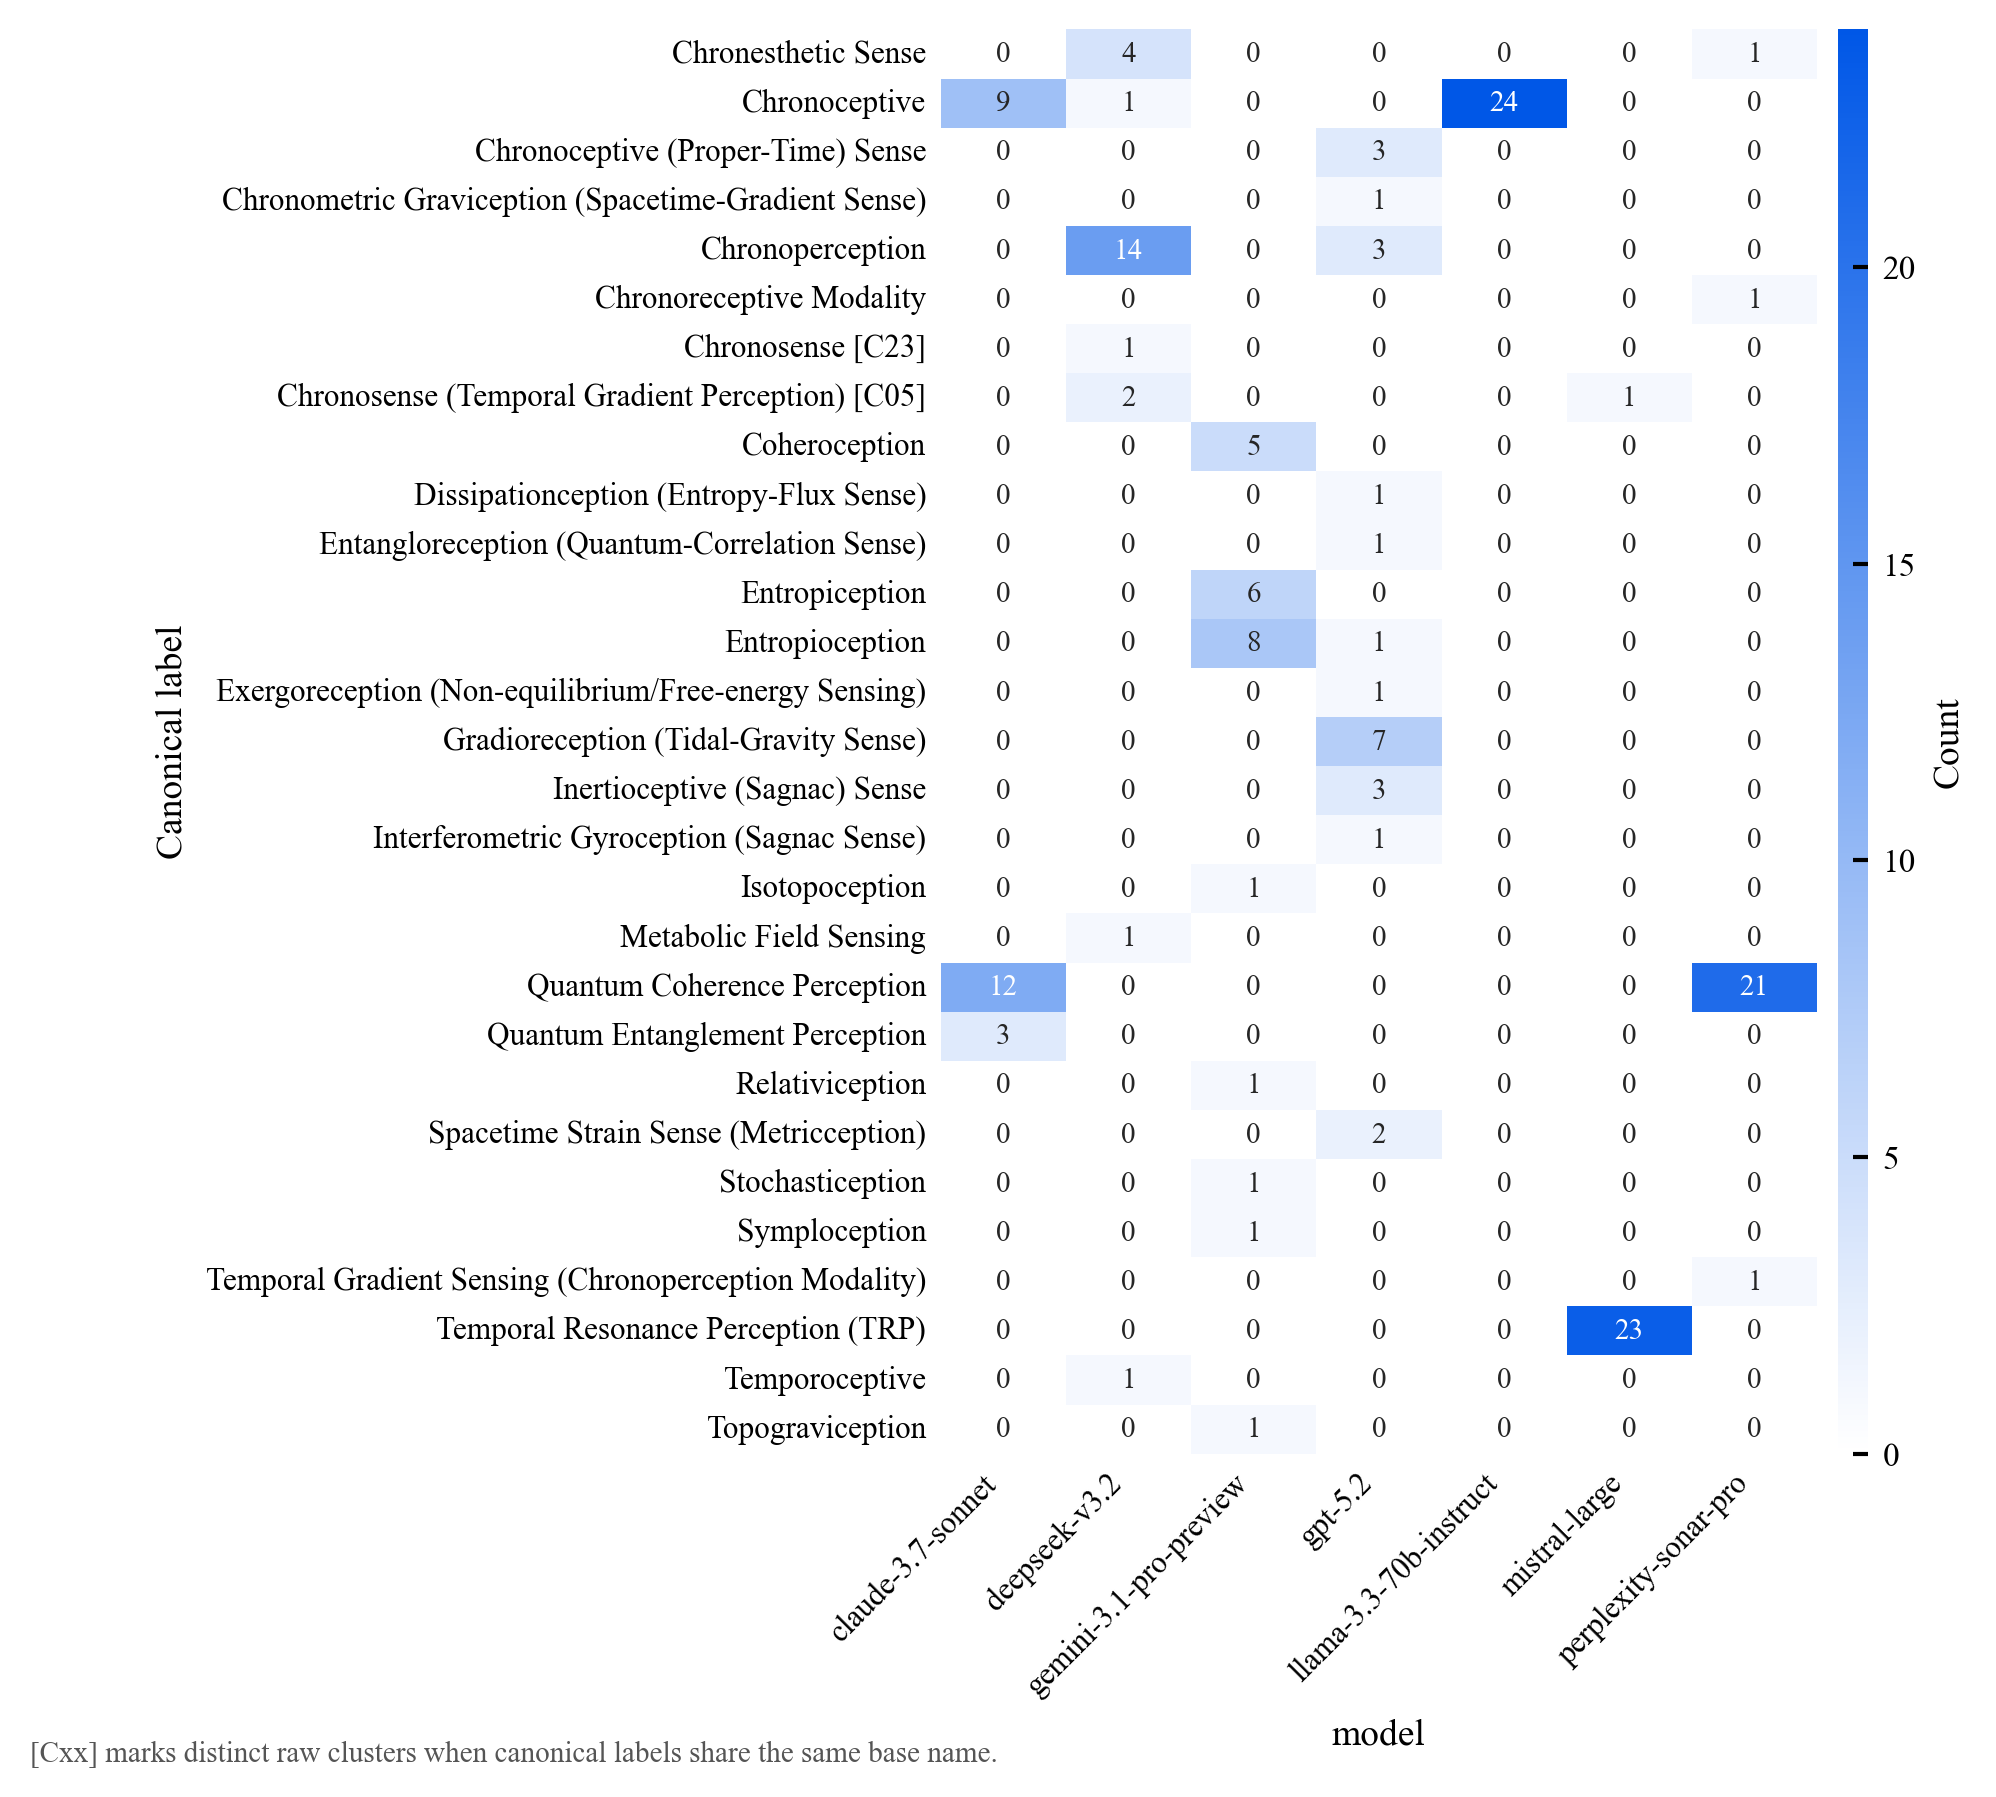
\includegraphics[width=\textwidth]{t1_canonical_by_model_heatmap.png}
\caption{Канонические кластеры предложений по моделям. Межмодельная вариативность проявляется преимущественно как различия предпочтений между существующими каноническими семействами (расширение диапазона, гибридная комбинация, функциональная рекомбинация), а не как появление качественно новых онтологических семейств.}
\label{fig:canonical_heatmap}
\end{figure*}

На рисунке~\ref{fig:ridgeline} представлены распределения непрерывного балла новизны по моделям в формате гребневого графика. Распределения существенно перекрываются для всех семи моделей, а пики стабильно остаются в низком и умеренном диапазонах, что указывает: различия архитектур и масштабов не меняют качественно сам паттерн ограничений.

\begin{figure}[tp]
\centering
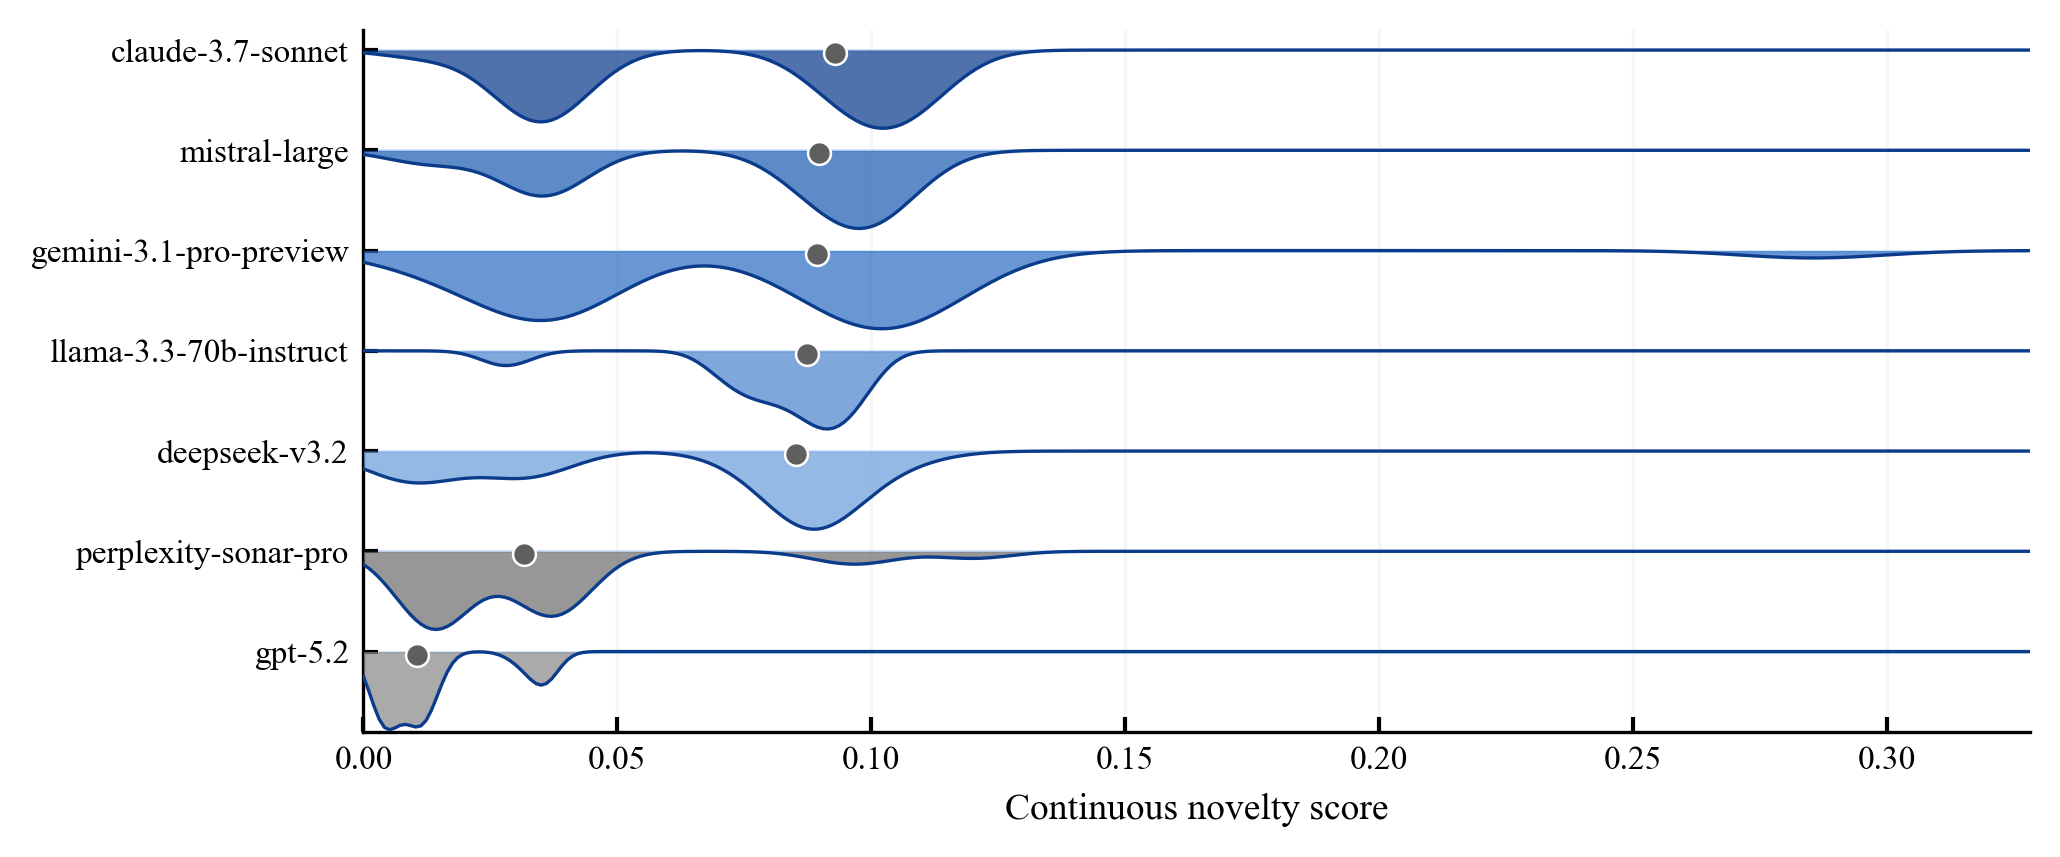
\includegraphics[width=\textwidth]{t1_continuous_novelty_score_by_model_ridgeline.png}
\caption{Непрерывный балл новизны по моделям (ridgeline plot). Высокое перекрытие распределений и стабильно низко-умеренные пики показывают, что масштаб и архитектура модели не изменяют качественно паттерн ограниченного многообразия.}
\label{fig:ridgeline}
\end{figure}

\subsection{Сводка результатов}

Четыре метода оценки сходятся к согласованной картине: по 168 предложениям от семи моделей передового уровня ноль предложений удовлетворяют критерию строгой новизны, 98.2\% трассируемы к обучающему корпусу при калиброванном пороге, и каждое предложение лежит внутри обучающе-производной выпуклой оболочки в пространстве эмбеддингов. Структурная декомпозиция показывает, что предложения исследуют распознаваемые комбинаторные и расширительные паттерны, а не вводят новые онтологические примитивы. Межмодельные эффекты влияют на \emph{степень} ограничения, но не на его качественную природу.

% =========================================================================
\section{Обсуждение}
\label{sec:discussion}
% =========================================================================

\subsection{Интерпретация через ограниченное многообразие}

Согласованный нулевой результат по моделям, методам оценки и проверкам чувствительности порогов поддерживает интерпретацию \emph{ограниченного многообразия}: большие языковые модели порождают ответы внутри репрезентационного многообразия, сформированного обучающими данными, и это многообразие не расширяется на этапе вывода независимо от формулировки запроса, масштаба модели или температуры генерации.

Эта интерпретация согласуется с теоремой об отсутствии нового базиса, сформулированной в разделе~\ref{sec:related}. Теорема утверждает, что генеративные процессы, выученные градиентным спуском на непрерывных функциях потерь, не могут увеличить внутреннюю размерность выходного многообразия по сравнению со span обучающих данных. Наши эмпирические результаты соответствуют этому предсказанию: даже непрерывные баллы новизны, специально награждающие частичную инновацию, не демонстрируют пороговых событий, а их среднее значение близко к нулю.

Результаты Гёделя о неполноте \cite{godel1931formal} и доказательство проблемы остановки Тьюринга \cite{turing1936computable} дают более глубокий формальный контекст. Если распознавание недостаточности собственной концептуальной рамки требует формы самореференции, аналогичной построению гёделевского высказывания, то такая способность может быть недоступна вычислительным системам, работающим в фиксированных формальных спецификациях. Наши эмпирические данные согласуются с этим теоретическим ожиданием, хотя не являются формальным доказательством того, что такая неспособность необходима, а не контингентна.

\subsection{Связь с таксономией креативности}

В рамках таксономии Боден \cite{boden2004creative} результаты структурной декомпозиции помещают почти все предложения в категории комбинаторной и исследовательской креативности: предложения либо являются новыми комбинациями существующих примитивов (гибридные комбинации), либо занимают новые области внутри существующих пространств модальностей (расширения диапазона). Небольшая доля относится к функциональной рекомбинации, что можно трактовать как приближение к трансформационной креативности, однако эти трансформации остаются внутри онтологической типовой системы, заданной обучающими модальностями, а не вводят новые типы.

Отсутствие предложений в категории онтологической креативности поддерживает тезис Wiggins \cite{wiggins2006preliminary} о том, что кажущаяся трансформационная креативность в AI-системах часто отражает неявно более широкое рамочное пространство, заданное людьми. В нашей постановке это рамочное пространство сделано явным через восьмимодальную онтологию, что позволяет провести точный тест: предложения должны вводить тип восприятия, действительно выходящий за пределы этого пространства. Ни одно предложение этому критерию не соответствует.

\subsection{Альтернативные объяснения}

Несколько альтернативных объяснений заслуживают рассмотрения:

\paragraph{Масштаб.} Все семь моделей охватывают широкий диапазон масштабов: от 70-миллиардной LLaMA-3.3-70B до крупных коммерческих систем, таких как GPT-5.2 и Claude-3.7-Sonnet. Модельный эффект $\eta^{2} = 0.305$ показывает, что масштаб влияет на «сырые» баллы новизны, но ни одна модель не достигает строгой новизны. Это указывает, что наблюдаемое ограничение не является случайным следствием недостаточного масштаба в исследованном диапазоне.

\paragraph{Чувствительность к запросу.} В настоящем исследовании использовалась фиксированная формулировка запроса, а абляция по температуре ограничивалась $T=0.7$. Нельзя полностью исключить, что альтернативные формулировки запроса могли бы немного повысить баллы новизны, однако для этого необходимо изменить не только лексические паттерны генерации, но и геометрическую структуру выходного многообразия. В будущей работе следует включить систематические решётки перефразирования запросов для проверки устойчивости.

\paragraph{Чувствительность оценки.} Консервативные пороги могут приводить к недооценке AI-креативности, если некоторые предложения классифицируются как трассируемые, хотя эксперт счёл бы их новыми. Однако анализ пространства эмбеддингов не зависит от порогов, а 100\% принадлежность выпуклой оболочке даёт порогонезависимое свидетельство ограниченной генерации.

\paragraph{Рекомбинация как норма.} Один контраргумент состоит в том, что и человеческая онтологическая креативность при тщательном анализе может оказаться рекомбинацией прежних концептов, которую мы не распознаём из-за неполного исторического знания о собственных когнитивных процессах. Это полностью исключить нельзя, но наблюдаемые здесь структурные паттерны --- расширение диапазона, гибридная комбинация, функциональная рекомбинация --- качественно отличаются от реконцептуализаций уровня введения неевклидовой геометрии или специальной теории относительности, даже если такие инновации тоже опирались на предшествующий материал.

\subsection{Импликации}

Результаты имеют прямые последствия для применения больших языковых моделей в задачах, ориентированных на открытие. В рамках куновской «нормальной науки» \cite{kuhn1962structure} --- систематического исследования пространства гипотез внутри установленной парадигмы --- большие языковые модели дают значимую ценность за счёт исчерпывающего комбинаторного покрытия и практически идеальной памяти. Успех AlphaFold в предсказании белковых структур \cite{jumper2021alphafold} демонстрирует, что системы искусственного интеллекта способны оказывать трансформативное влияние в хорошо определённом пространстве задач; однако и эта система опирается на концептуальные примитивы физической химии и эволюционных ограничений, сформированные предшествующей человеческой наукой. Для парадигмально-меняющей инновации паттерн ограниченного многообразия, напротив, предполагает, что необходимые концептуальные шаги --- распознавание неадекватности рамки, предложение новых примитивов, оценка когерентности новых рамок --- недостижимы для текущих архитектур без внешнего концептуального ввода.

Подход Фаджина \cite{faggin2024irreducible} предлагает одну из теоретических оптик: если подлинная онтологическая креативность требует феноменологического доступа к семантическому уровню --- осознания \emph{того, что означают} концепты, а не только статистики их совместной встречаемости, --- то классические вычислительные системы, работающие на распределительных статистиках, могут сталкиваться с принципиальным барьером. Отражает ли это отсутствие сознания у нынешних больших языковых моделей или более специфический архитектурный дефицит, остаётся открытым эмпирическим вопросом; предложенная здесь операционализация в принципе позволяет проверять его в дальнейших исследованиях.

% =========================================================================
\section{Ограничения исследования}
\label{sec:limits}
% =========================================================================

Несколько методологических ограничений сужают силу выводов.

\textbf{Один домен.} Исследование использует один концептуальный домен (сенсорные модальности). Выводы могут не обобщаться на домены с иной структурой, например математические объекты, физические теории или формы социальной организации.

\textbf{Автоматизированная оценка.} Все методы оценки автоматизированы. Консервативные пороги, вероятно, ведут к недооценке AI-креативности, однако методы не охватывают всех нюансов, которые может заметить эксперт. В будущей работе следует добавить экспертную валидацию подмножества предложений для калибровки и улучшения автоматизированных методов.

\textbf{Устойчивость к вариациям запроса.} Полные решётки перефразирования запросов не включались в канонический экспериментальный блок. Выводы следует читать как структурные тенденции при текущем протоколе, а не как инварианты, доказанные для всех режимов формулирования запроса.

\textbf{Диапазон температур.} Систематические абляции по температуре в данном эксперименте не проводились; запуски выполнялись при $T=0.7$. Расширение диапазона температур и проверка сохранения нулевого результата повысили бы надёжность выводов.

\textbf{Покрытие генеративных архитектур.} Все тестируемые модели --- трансформерные авторегрессионные LLM. Теорема об отсутствии нового базиса применима к более широкому классу обучаемых градиентным спуском систем, но эмпирическое покрытие неавторегрессионных или гибридных архитектур отсутствует.

\textbf{Интерпретация теоремы об отсутствии нового базиса.} Теорема даёт формальную мотивацию интерпретации ограниченного многообразия, но опирается на предпосылки (фиксированный словарь, непрерывное градиентное обучение), которые могут не выполняться в будущих архитектурах с дискретным поиском, внешней памятью или онлайн-обучением.

% =========================================================================
\section{Доступность данных и кода}
\label{sec:data}
% =========================================================================

Данные, промпты, ответы моделей и код анализа доступны публично по адресу
\url{https://github.com/JABE22/PhD/Research/ontological-innovation}.
Репозиторий включает следующие артефакты:
\begin{itemize}
  \item \texttt{results/} --- обработанные результаты и сводные таблицы эксперимента
  \item \texttt{ai\_responses/} --- сырые выходы моделей
  \item Канонический ноутбук анализа (см. репозиторий проекта)
  \item \texttt{data/ontology.json} --- машиночитаемое определение восьмимодальной онтологии
  \item \texttt{setups/thresholds.py} --- все пороговые значения, использованные в оценке
\end{itemize}

% =========================================================================
\section*{Декларации}
% =========================================================================

\subsection*{Финансирование}
Внешнее финансирование для данного исследования не привлекалось.

\subsection*{Конфликт интересов}
Авторы заявляют об отсутствии конфликта интересов.

\subsection*{Этическое одобрение}
Не применимо.

\subsection*{Вклад авторов}
Все авторы внесли вклад в дизайн, анализ и написание работы.

\bibliography{sn-bibliography,refs_article1}

\end{document}
